
\section{Experiments}

\noindent \textbf{Main results.} The speed of \our is approximately $\textbf{2.1}\times$ faster than FlashAttention-2. Furthermore, \our achieves an average real speedup of $\textbf{2.83}\times$ compared to the original attention in various models, with \textbf{negligible loss in end-to-end metrics}.

\subsection{Experimental Setup} \label{sec:exp_set_up}

\noindent \textbf{Models.} 
%
We validate the effectiveness of \our across a diverse set of representative models from the fields of language, image, and video generation.
Specifically, we conduct experiments on five models: \llama(7B)~\citep{touvron2023llama2} for text2text, \cogvideo~\citep{yang2024cogvideox} for text2video, \unidiffuser~\citep{bao2022uni} and \ultrapixel~\citep{ren2024ultrapixel} for text2image, \timm~\citep{rw2019timm} for image classification, \purple{and \llava~\citep{liu2024llavanext} for visual question answering.}

\noindent \textbf{Datasets.}   
\llama is evaluated on three zero-shot tasks: WikiText~\citep{merity2022pointer} to assess the model's prediction confidence, LAMBADA~\citep{paperno2016lambada} evaluate contextual understanding, and MMLU~\citep{2020mmlu} for measuring knowledge across various subjects.
\cogvideo is evaluated using the open-sora~\citep{opensora} prompt sets.
Both \ultrapixel and \unidiffuser are assessed on the COCO annotations~\citep{lin2014microsoft}, featuring (prompt, image) pairs.
\timm is evaluated on on three image datasets: ImageNet~\citep{deng2009imagenet}, ImageNet-Sketch (Sketch)~\citep{wang2019sketch}, and ImageNet-Rendition (ImageNet-r)~\citep{hendrycks2021rendition}. \purple{\llava is evaluated on three datasets: TextVQA~\citep{singh2019towards}, POPE~\citep{li2023evaluating}, and VQAv2~\citep{goyal2017making}.}


\noindent \textbf{Metrics.}   
For \llama, we use perplexity (ppl.)~\citep{jelinek1977perplexity} for WikiText, and Accuracy (Acc.) for LAMBADA and MMLU.
For \cogvideo, folowing~\citep{zhao2024vidit}, we evaluate the quality of generated videos on five metrics: CLIPSIM and CLIP-Temp (CLIP-T)~\citep{liu2024evalcrafter} to measure the text-video alignment; (VQA-a) and (VQA-t) to assess the video aesthetic and technical quality, respectively; and Flow-score (FScore) for temporal consistency~\citep{wu2023exploring}. 
For \ultrapixel and \unidiffuser, generated images are compared with the images in the COCO annotations dataset in three aspects: FID~\citep{heusel2017gans} and sFID~\citep{salimans2016improved} for fidelity evaluation, \textit{Clipscore} (CLIP)~\citep{hessel2021clipscore} for text-image alignment, and \textit{ImageReward} (IR)~\citep{xu2024imagereward} for human preference.
For \timm and \llava, we use Accuracy.



\begin{figure}[htb!]
    \centering
    \vspace{-.2em}
    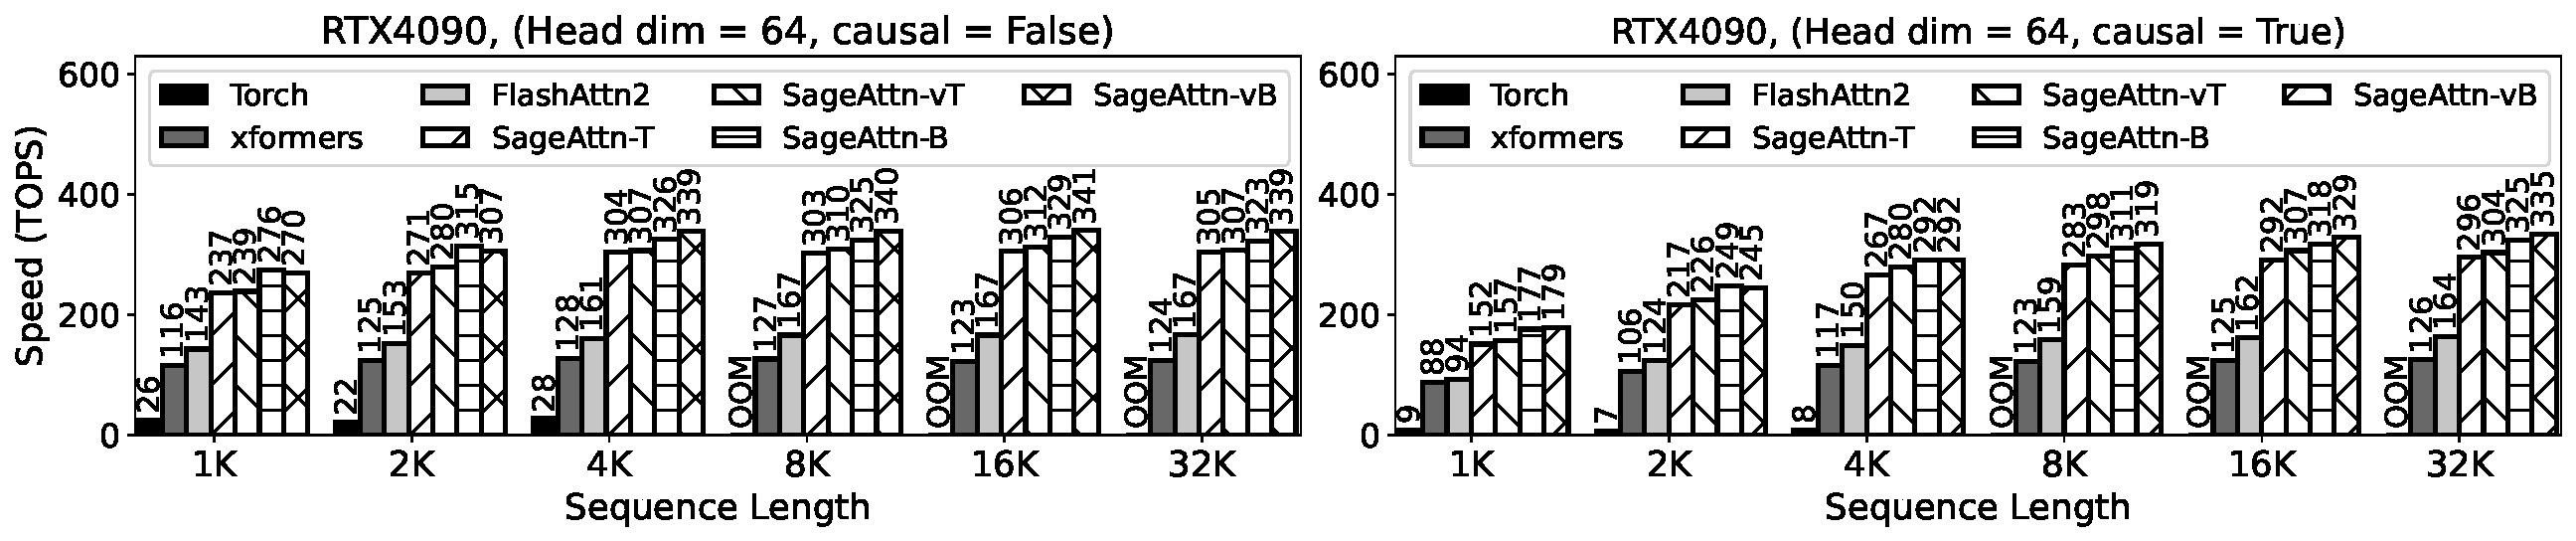
\includegraphics[width=1.0\textwidth]{figs/hd64_baselines_kernel_flops.pdf}
    \vspace{-1.8em}
    \caption{Speed comparison between \our and baselines (RTX4090, headdim=64).}
    \vspace{-.5em}
    \label{fig:kf_h64_baseline}
\end{figure}

\begin{figure}[htb!]
    \centering
    \vspace{-.2em}
    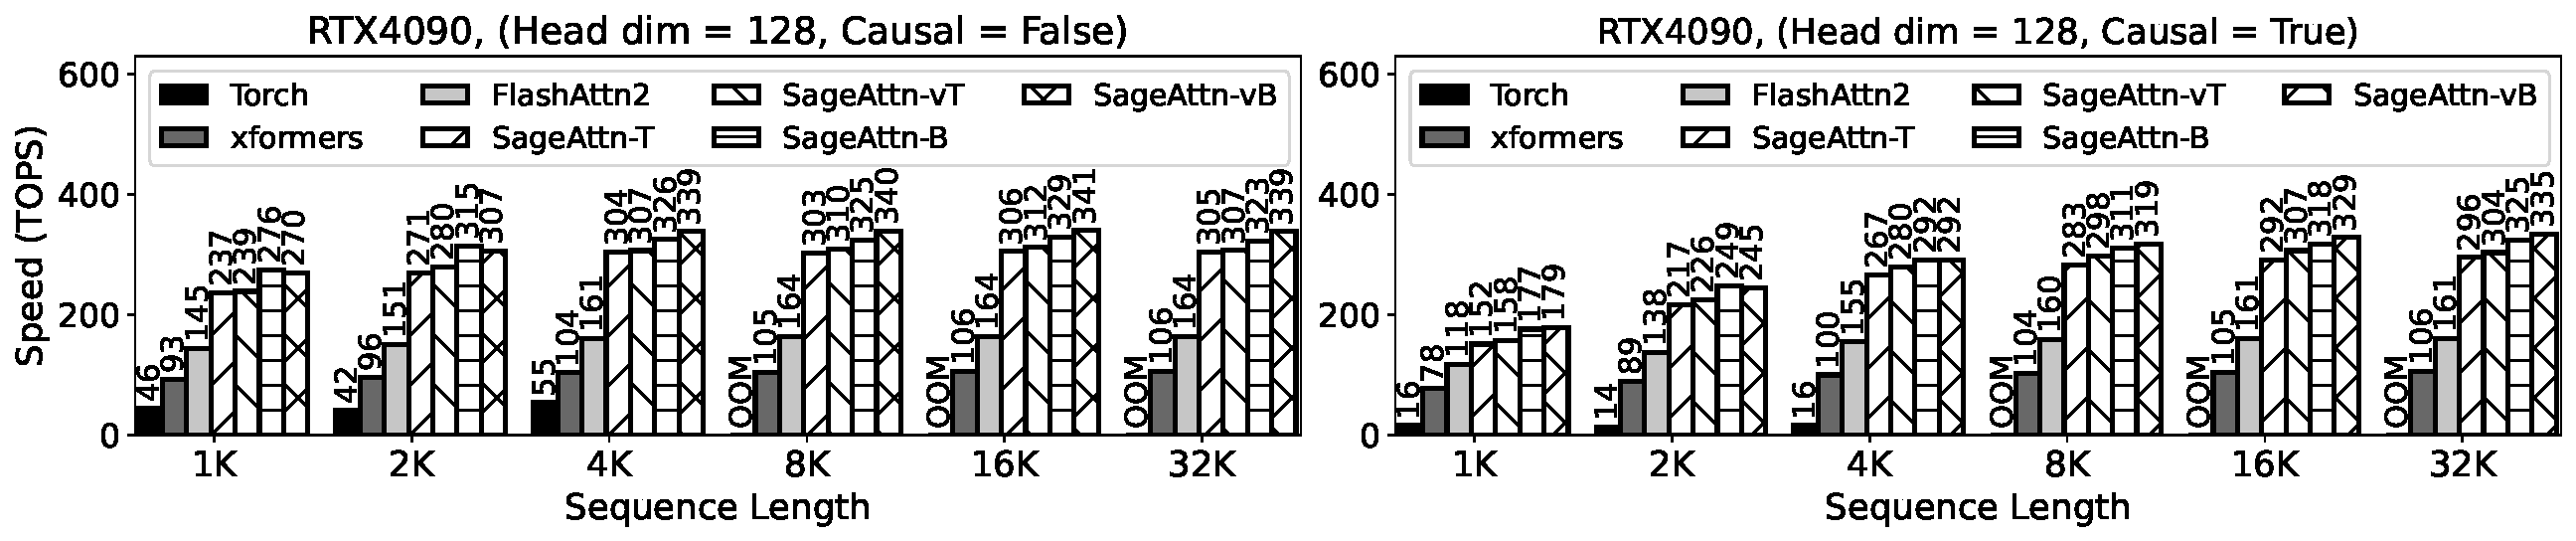
\includegraphics[width=1.0\textwidth]{figs/hd128_baselines_kernel_flops.pdf}
    \vspace{-1.8em}
    \caption{Speed comparison between \our and baselines (RTX4090, headdim=128).}
    \vspace{-.5em}
    \label{fig:kf_h128_baseline}
\end{figure}

\begin{figure}[htb!]
    \centering
    \vspace{-.2em}
    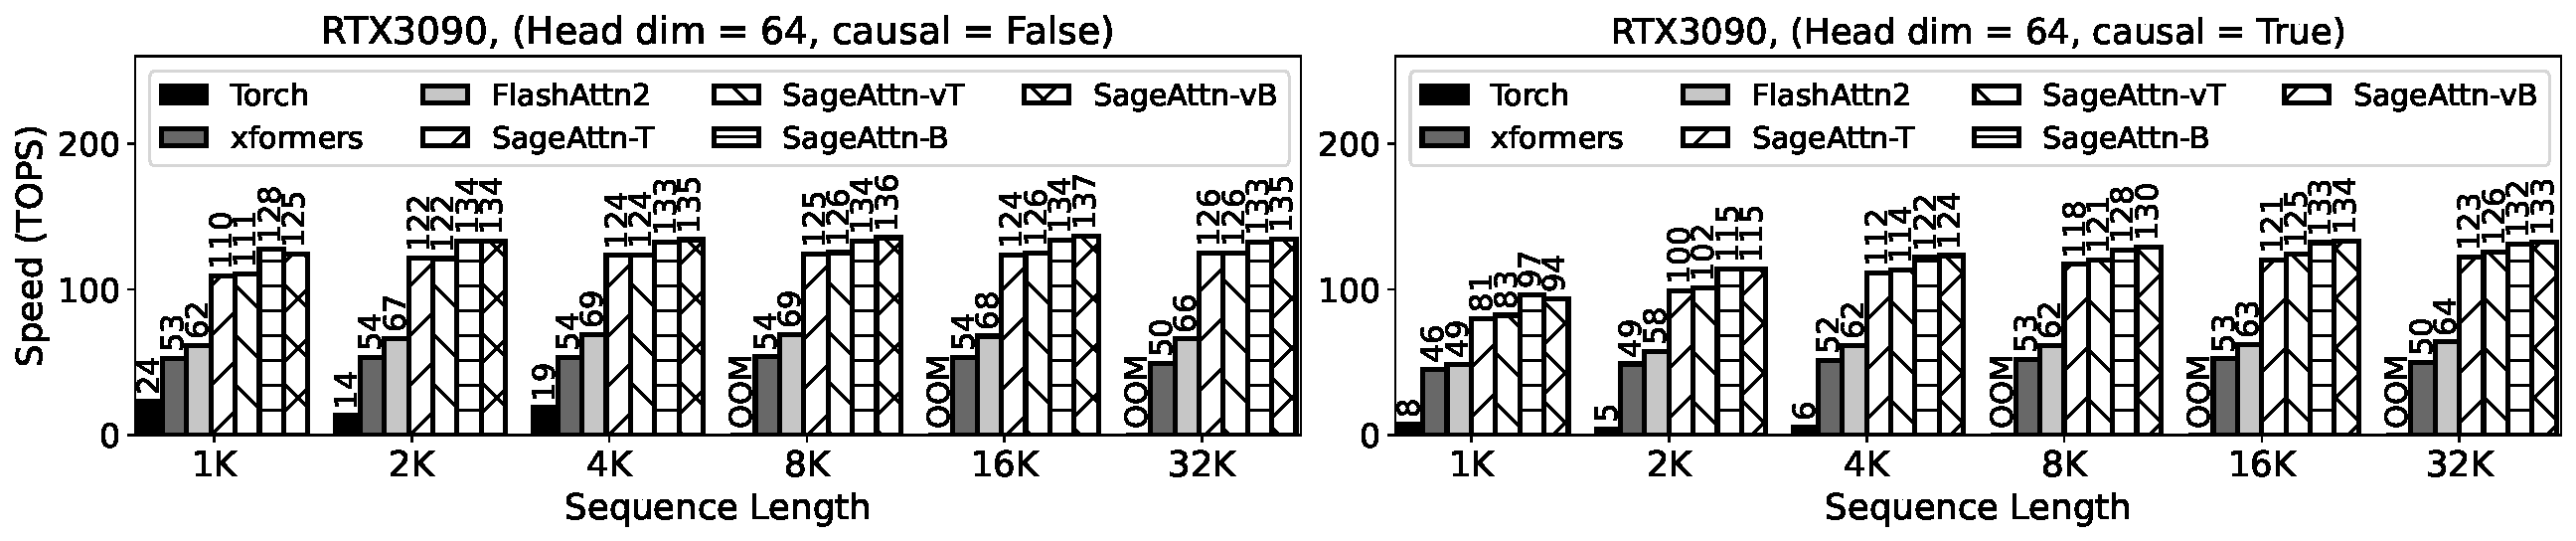
\includegraphics[width=1.0\textwidth]{figs/3090_hd64_baselines_kernel_flops.pdf}
    \vspace{-1.8em}
    \caption{Speed comparison between \our and baselines (RTX3090, headdim=64).}
    \vspace{-.5em}
    \label{fig:kf_h64_baseline_3090}
\end{figure}

\begin{figure}[htb!]
    \centering
    \vspace{-.2em}
    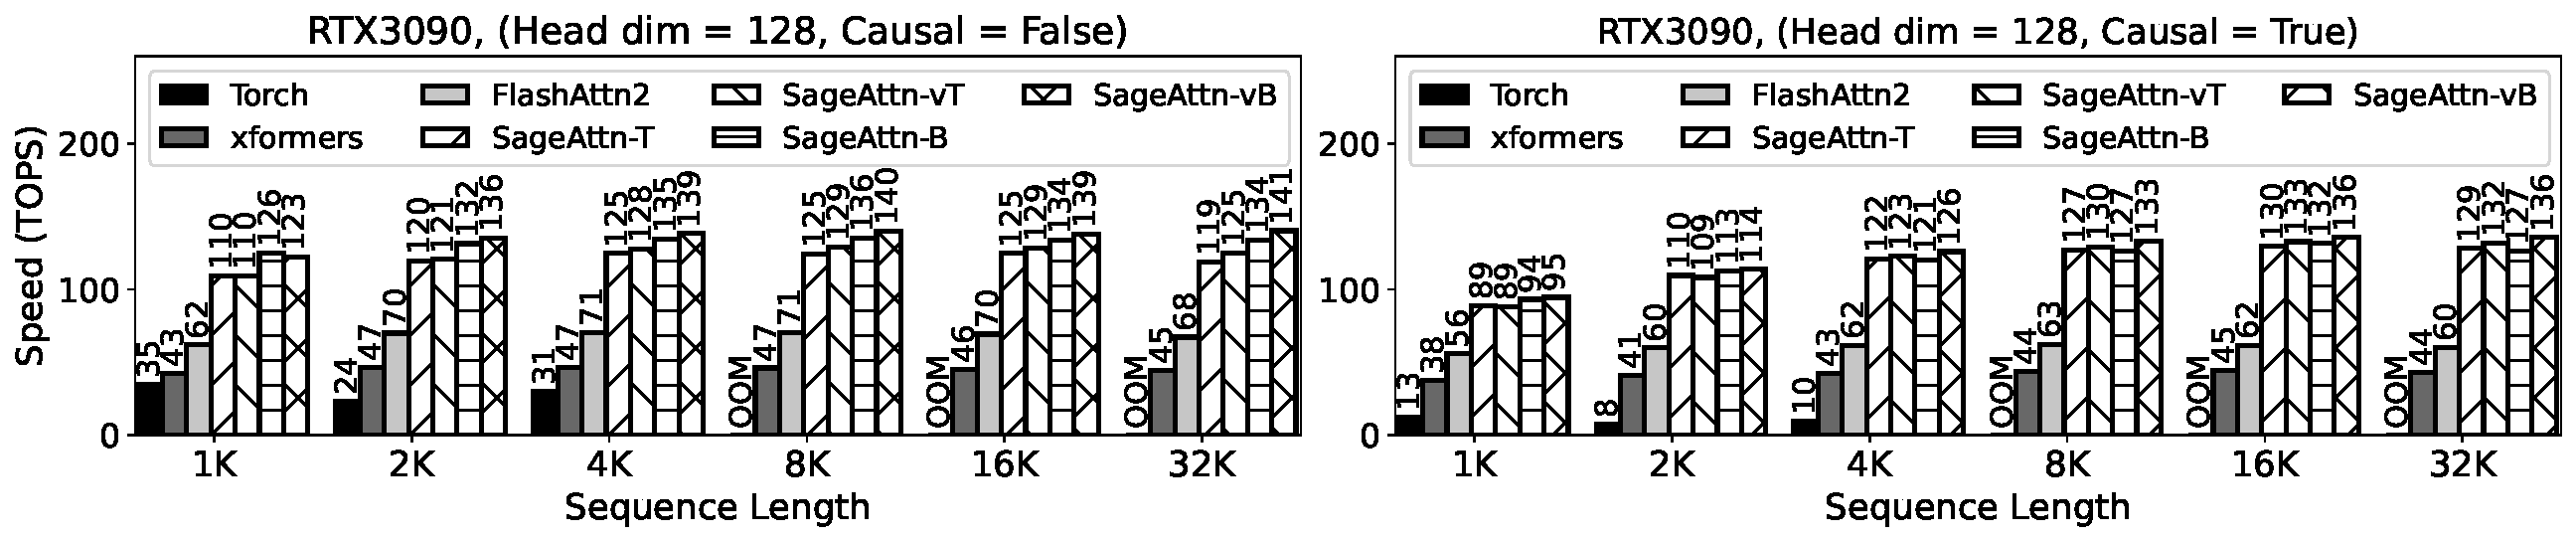
\includegraphics[width=1.0\textwidth]{figs/3090_hd128_baselines_kernel_flops.pdf}
    \vspace{-1.8em}
    \caption{Speed comparison between \our and baselines (RTX3090, headdim=128).}
    \label{fig:kf_h128_baseline_3090}
\vspace{.2em}
\end{figure}







\subsection{Speed and Accuracy of attention Kernels}

\noindent \textbf{Speed.} We conduct experiments to compare the Speed of \our against baselines using configurations with headdim=64 or headdim=128, both with and without Causal Mask~\cite{vaswani2017attention}. Specifically, Figure~\ref{fig:kf_h64_baseline} and Figure~\ref{fig:kf_h128_baseline} show the Speed of \our and baselines across varying sequence lengths on RTX4090. These results indicate that \our achieves a peak of \textbf{341} TOPS and is \textbf{2x} faster than FlashAttention2 and \textbf{2.9x} faster than xformers on average.
Figure~\ref{fig:kf_h64_baseline_3090} and Figure~\ref{fig:kf_h128_baseline_3090} illustrate the results on RTX3090, showing a similar speedup performance.



\noindent \textbf{Accuracy.} 
Table~\ref{tab:error of sage} shows the numerical error of four implementations of \our compared with attention in full-precision. This experiment is conducted using a set of (Q, K, V) conforming to a normal distribution. It shows the error of the four implementations is rather small. \ourt and \ourb achieve 100\% cosine similarity and RMSE in the e-4 level.




\begin{table}[htb!]
\vspace{-.2em}
    \caption{Real speedup of \our on RTX4090.}
    \label{exp:real_flops}
    \setlength\tabcolsep{6.5pt}
    \begin{center}
    \begin{tabular}{l|c|l|c|c}
    \toprule
    {\bf Model}  & {\bf Shape of Q, K, V}  & {\bf Original attention}  & {\bf SageAttention}  & {\bf Speedup}
    \\ \hline
    \cogvideo    & (2, 30, 17776, 64) &  163.37 (FlashAttn2)  &  \cellcolor{gray!20}\textbf{327.57}  & \cellcolor{gray!21}\textbf{2.01x}  \\
    \llama       & (4, 32, 1536, 128) &  130.99 (FlashAttn2)  &  \cellcolor{gray!20}\textbf{231.74}  & \cellcolor{gray!21}\textbf{1.77x}  \\ 
    \ultrapixel  & (2, 32, 7285, 64)  &  152.03 (FlashAttn2)  &  \cellcolor{gray!20}\textbf{325.18}  & \cellcolor{gray!21}\textbf{2.14x}  \\ 
    \unidiffuser & (4, 24, 1105, 64)  &  105.68 (xformers)    &  \cellcolor{gray!20}\textbf{246.93}  & \cellcolor{gray!21}\textbf{2.34x}  \\ 
    \timm        & (12, 64, 197, 64)  &  18.910 (Torch)       &  \cellcolor{gray!20}\textbf{111.41}  & \cellcolor{gray!21}\textbf{5.89x}  \\ \bottomrule
    \end{tabular}
    \end{center}
\vspace{-.2em}
\end{table}


\begin{table}[htb!]
    \caption{End-to-end metrics loss across text, image, and video generation models.}
    \label{exp:metrics_loss_t2t}
    \setlength\tabcolsep{4.25pt}
    \begin{center}
    \begin{tabular}{p{2.1cm}|p{2.55cm}|c|c|c}
    \toprule
    {\bf Model}  & {\bf Attention}  & {\bf WikiText (Ppl.) $\downarrow$}  & {\bf Lambda (Acc.) $\uparrow$}  & {\bf MMLU (Acc.) $\uparrow$}  \\ \hline
    \multirow{2}{*}{\llama} & Full-Precision & 5.823 & 0.886  & 0.46   \\  % \cline{2-5}
    & \cellcolor{gray!24}\textbf{SageAttention} & \cellcolor{gray!24}\textbf{\dgreen{5.824}} &  \cellcolor{gray!24}\textbf{\dgreen{0.887}}  & \cellcolor{gray!24}\textbf{\dgreen{0.46}}   \\ \bottomrule
    \end{tabular}
    \end{center}
    
    \begin{center}
    \setlength\tabcolsep{3.6pt}
    \begin{tabular}{p{2.2cm}|p{2.55cm}|c|c|c|c|c}
    \toprule
    {\bf Model}  & {\bf Attention}  & {\bf CLIPSIM $\uparrow$}  & {\bf CLIP-T $\uparrow$}  & {\bf VQA-a $\uparrow$}  & {\bf VQA-t $\uparrow$}  & {\bf FScore $\uparrow$} \\ \hline
    \multirow{2}{*}{\cogvideo} & Full-Precision & 0.1837 & 0.9976  & 68.962  & 75.925  &  3.7684  \\  % \cline{2-7}
    & \cellcolor{gray!24}\textbf{SageAttention} & \cellcolor{gray!24}\textbf{\dgreen{0.1836}} &  \cellcolor{gray!24}\textbf{\dgreen{0.9976}}  & \cellcolor{gray!24}\textbf{\dgreen{68.839
    }}  &  \cellcolor{gray!24}\textbf{\dgreen{75.037}}  &  \cellcolor{gray!24}\textbf{\dgreen{3.8339}} \\ \bottomrule
    \end{tabular}
    \end{center}
    
    \begin{center}
    \setlength\tabcolsep{15.5pt}
    \begin{tabular}{p{1.4cm}|p{1.725cm}|c|c|c|c}
    \toprule
    {\bf Model}  & {\bf Attention}  & {\bf FID $\downarrow$}  & {\bf sFID $\downarrow$}  & {\bf CLIP $\uparrow$}  & {\bf IR $\uparrow$}
    \\ \hline
    \multirow{2}{*}{\hspace{-1.2em}\unidiffuser} & \hspace{-1.2em}Full-Precision & 163.33 & 145.08  & 0.3152  & 0.1609  \\  % \cline{2-6} 
    & \cellcolor{gray!24}\hspace{-1.2em}\textbf{SageAttention} &  \cellcolor{gray!24}\textbf{\dgreen{166.49}} & \cellcolor{gray!24}\textbf{\dgreen{143.18}}  & \cellcolor{gray!24}\textbf{\dgreen{0.3154}}  &  \cellcolor{gray!24}\textbf{\dgreen{0.1521}} \\ \hline
    \multirow{2}{*}{\hspace{-1.2em}\ultrapixel} & \hspace{-1.2em}Full-Precision & 179.78 & 141.35  & 0.3132  & 0.6169  \\  % \cline{2-6}
    & \cellcolor{gray!24}\hspace{-1.2em}\textbf{SageAttention} & \cellcolor{gray!24}\textbf{\dgreen{179.79}} &  \cellcolor{gray!24}\textbf{\dgreen{141.63}} & \cellcolor{gray!24}\textbf{\dgreen{0.3131}}  &  \cellcolor{gray!24}\textbf{\dgreen{0.6110}} \\ \bottomrule
    \end{tabular}
    \end{center}


    
    \begin{center}
    \setlength\tabcolsep{2.3pt}
    \begin{tabular}{p{2.35cm}|p{2.65cm}|c|c|c}
    \toprule
    {\bf Model}  & {\bf Attention}  & {\bf ImageNet (Acc.) $\uparrow$}  & {\bf Sketch (Acc.) $\uparrow$}  & {\bf ImageNet-r (Acc.) $\uparrow$}  \\ \hline
    \multirow{2}{*}{\timm} & Full-Precision &  84.79\% & 45.32\%  & 59.55\%   \\  % \cline{2-5}
            & \cellcolor{gray!24}\textbf{SageAttention} & \cellcolor{gray!24}\textbf{\dgreen{84.74\%}}  &  \cellcolor{gray!24}\textbf{\dgreen{45.78\%}}  & \cellcolor{gray!24}\textbf{\dgreen{60.32\%}}   \\ \bottomrule
    \end{tabular}
    \end{center}

    \begin{center}
    \setlength\tabcolsep{5.65pt}
    \begin{tabular}{p{2.15cm}|p{2.4cm}|c|c|c}
    \toprule
    {\bf Model}  & {\bf Attention}  & {\bf TextVQA (Acc.) $\uparrow$}  & {\bf POPE (Acc.) $\uparrow$}  & {\bf VQAv2 (Acc.) $\uparrow$}  \\ \hline
    \multirow{2}{*}{\llava} & Full-Precision & 60.25\% & 86.45\%  & 77.55\%   \\  % \cline{2-5}
            & \cellcolor{gray!24}\textbf{SageAttention} & \cellcolor{gray!24}\textbf{\dgreen{60.09\%}}  &  \cellcolor{gray!24}\textbf{\dgreen{86.44\%}}  & \cellcolor{gray!24}\textbf{\dgreen{77.47\%}}   \\ \bottomrule
    \end{tabular}
    \end{center}
\end{table}
\vspace{-1em}




\subsection{End-to-end Performance}
\textbf{Speedup.} We measure the real speed of \our and the original attention on \unidiffuser, \ultrapixel, \cogvideo, \llama and \timm on RTX4090. 
Table~\ref{exp:real_flops} shows that \our outperforms original attention across all models. Specifically, \our yields \textbf{2.83x} speedup compared to the original attentions on average.

\textbf{Metrics loss.} We assessed the end-to-end metrics of various models using \our compared to using attention in full-precision.
Detailed evaluation results are presented in Table~\ref{exp:metrics_loss_t2t} for \llama, \cogvideo, \unidiffuser, \ultrapixel, and \timm, respectively. The results indicate that \our successfully matches the performance of attention in full-precision across all models. Specifically, on \llama, \cogvideo, \ultrapixel, and \unidiffuser, \our resulted in only a minor average degradation of 0.2\% compared to attention in full-precision. Moreover, on \timm, \our even surpasses attention in full-precision.


\begin{table}[htb!]
\vspace{-1.3em}
    \centering
    \begin{minipage}{0.54\textwidth}
        \raggedright
        \caption{Accuracy of SageAttention kernels.}
        \label{tab:error of sage}
        \setlength\tabcolsep{2.7pt}
        \scalebox{0.95}{
        \begin{tabular}{c||c|c|c}
            \toprule
            {\bf attention}  & {\bf Cos Sim $\uparrow$}  & {\bf Relative L1 $\downarrow$}  & {\bf RMSE $\downarrow$}  \\ \hline
            \ourt   &   1.0    & 0.019  & 6.8e{-4}  \\ 
            \cellcolor{gray!24}\ourb   &   \cellcolor{gray!24}1.0   & \cellcolor{gray!24}0.021  & \cellcolor{gray!24}7.3e{-4}  \\ 
            \ourvt  &  99.9\%   & 0.064  & 0.065  \\ 
            \ourvb  &  98.9\%   & 0.138  & 0.067  \\ \bottomrule
        \end{tabular}
        }
    \end{minipage}
    \hspace{0.03\textwidth} 
    \begin{minipage}{0.39\textwidth}
        \raggedleft
        \caption{Overhead of smoothing K.}
        \label{exp:overhead_km}
        \setlength\tabcolsep{3pt}
        \scalebox{0.95}{
        \begin{tabular}{l|c|c}
        \toprule
        {\bf Model}  & {\bf Smooth K}  & {\bf TOPS $\uparrow$} \\
        \hline
        \multirow{2}{*}{\cogvideo} &  \ding{55}  & 327.57 \\
                                    & \cellcolor{gray!24}\checkmark  & \cellcolor{gray!24}\textbf{327.52} \\ \hline
        \multirow{2}{*}{\ultrapixel} & \ding{55}  & 325.18 \\
                                    & \cellcolor{gray!24}\checkmark  & \cellcolor{gray!24}\textbf{324.56} \\ 
        \bottomrule
        \end{tabular}
        }
    \end{minipage}
\end{table}



\begin{table}[h!]
\vspace{-1.5em}
    \caption{Benefit of adaptive quantization.}
    \label{exp:adaptive_quant}
    \setlength\tabcolsep{3.9pt}
    \begin{center}
    \scalebox{0.96}{
    \begin{tabular}{l||l|c|c||l|c|c}
    \toprule
    {\bf attention}  & {\bf model}  & {\bf CLIPSIM $\uparrow$} & {\bf TOPS $\uparrow$}  & {\bf Model} & {\bf MMLU $\uparrow$} & {\bf TOPS $\uparrow$}    \\ \hline
    \ourt  & \multirow{2}{*}{\cogvideo} &  0.1827  &  292.17 & \multirow{2}{*}{\llama}  & 0.46   &  208.59 \\  % \cline{2-5}
    \cellcolor{gray!24}\our   &   & \cellcolor{gray!24}\textbf{0.1835}  & \cellcolor{gray!24}\textbf{327.57}  &   &  \cellcolor{gray!24}\textbf{0.46}   &  \cellcolor{gray!24}\textbf{231.74} \\ \bottomrule
    \end{tabular}
    }
    \end{center}
    \vspace{-1.2em}
\end{table}



\subsection{Ablation Study}
\vspace{-.75em}
\textbf{Overhead of smoothing K.} Table~\ref{exp:overhead_km} presents the overhead associated with smoothing K on the attention speed in real models. The results indicate a minimal reduction, less than 0.2\%.



\textbf{Benefit of adaptive quantization.} We analyzed the performance differences between using only \ourt and employing an adaptive strategy (\our). Table~\ref{exp:adaptive_quant} presents the metrics and average speed of attention on \cogvideo and \llama. The results indicate that the adaptive strategy increases the speed of attention by 11.7\% without any loss in metrics.

